%!TEX root =  main.tex



\section{Analysis of the ODA Algorithm (Algorithm \ref{alg:decen}) }\label{sec:oda:appendix}






\subsection{Proof of Theorem \ref{thm:decen} }\label{sec:proof:decen}

We first provide a proof sketch of Theorem \ref{thm:decen} and the detailed proof is presented later. 






\paragraph{Proof Sketch}\label{sec:proof:sketch}
We first show that, with high probability, the real preference value $\mu_{i,j}$ can be upper bounded by $\ucb_{i,j}(t)$ and lower bounded by $\lcb_{i,j}(t)$ in each round $t$. In the following, we would analyze the algorithm based on this high-probability event. 

At a high level, Algorithm \ref{alg:decen} can be regarded as an online version of DA. 
In DA with arm proposing, at each step, each arm $a_j$ proposes to the player set $\ch_j(P_{i,j})$, which is equivalent in our algorithm to each player $p_i$ proposing arms in the plausible set constructed as $S_i(t)=\set{a_j\in \cK: p_i \in \ch_j(P_{i,j})}$.
Then each player would reject all but the most preferred arm among those who propose to it, equivalent in our algorithm to players deleting all arms in the plausible set but the one with the highest preference value. 
But since players do not know their own preferences in our setting, they need to explore these arms to learn the corresponding preference values. 
Based on the above high-probability event and the construction of the two confidence bounds, if $\mu_{i,j}<\mu_{i,j'}$ for player $p_i$ and arms $a_j,a_{j'}$ in its plausible set, these two arms would be selected by $p_i$ for at most $O(\log T/\Delta^2_{i,j,j'})$ times before $\ucb_{i,j}<\lcb_{i,j'}$ and further arm $a_j$ is considered to be less preferred than other plausible arms. 
We can regard this event as $p_i$ rejects arm $a_j$ in DA. 
When all players determine the most-preferred arm from the plausible set, the corresponding DA can proceed to the next step and arms then propose the preferred subset of players among those who have not rejected them. 
In the offline DA algorithm, the rejection can happen for at most $NK$ times since each player can reject each arm at most once. 
Correspondingly, the regret of our algorithm is at most $O(NK\log T/\Delta^2)$ before reaching stability. 







\subsubsection{Full Proof}\label{sec:proof:full}



In this section, we provide the detailed proof of Theorem \ref{thm:decen}. 




Let $P_{i,j}(t)$ be the value of $P_{i,j}$ at the end of round $t$.
Recall $\bar{A}(t)=\set{(p_i,\bar{A}_i(t)):p_i\in \cN}$ is the matching at round $t$ and $M^*$ is the set of all stable matchings. Further, denote $A(t)=\set{(p_i,A_i(t)):p_i\in \cN}$ as the set of players and their selected arms at round $t$.  
The player-pessimal stable regret of $p_i$ can then be bounded by 
\begin{align}
    \underline{R}_i(T) &\le  \EE{\sum_{t=1}^T \bOne{\bar{A}(t) \notin M^* }}\cdot \mu_{i,\underline{m}_i} \notag\\
    &= \EE{\sum_{t=1}^T \bOne{{A}(t)  \notin M^* }}\cdot \mu_{i,\underline{m}_i} \label{eq:decen:nocollision} \\
    &\le \EE{\sum_{t=1}^T \bOne{{A}(t) \notin M^*  } \mid \urcorner \cF }\cdot \mu_{i,\underline{m}_i} + T\cdot \PP{ \cF}\cdot \mu_{i,\underline{m}_i} \notag \\
    &\le \bracket{\frac{192NK\log T}{\Delta^2} + 2NK} \mu_{i,\underline{m}_i} + 2NK\mu_{i,\underline{m}_i} \label{eq:decen:main and badevent}  \\
    &= O\bracket{NK\log T/\Delta^2} \notag \,,
\end{align}

where Eq.\eqref{eq:decen:nocollision} holds according to Lemma \ref{lem:decen:nocollision}, Eq.\eqref{eq:decen:main and badevent} comes from Lemma \ref{lem:cen:badevent} and Lemma \ref{lem:decen:mainevent}. 






\begin{lemma}\label{lem:decen:nocollision}
In Algorithm \ref{alg:decen}, at each round $t$, $\bar{A}_i(t) = A_i(t)$ for each player $p_i$. 
\end{lemma} 
\begin{proof}
The case where $A_i(t) = \emptyset$ holds trivially. In the following, we mainly consider the case where $A_i(t) \neq \emptyset$. 

According to Lemma \ref{lem:decen:sameP}, all players have the same $P_{i,j}(t)$ at each time $t$ for each arm $a_j$. For simplicity, we then set $P_j(t) = P_{i,j}(t)$ for any arm $a_j$ and $p_i \in \cN$. In Algorithm \ref{alg:decen}, when player $p_i$ proposes to $A_i(t) =a_j \in S_i(t)$, we have $p_i \in \ch_j(P_j(t-1))$. 
Thus it holds that $A^{-1}_j(t)\subseteq \ch_j(P_j(t-1))$. 
According to the substitutability, for each player $p_i$ who proposes to $a_j$, $p_i \in \ch_j(P_j(t-1)\cap A^{-1}_j(t)) = \ch_j(A^{-1}_j(t))$. According to the acceptance protocol of the arm side, each $p_i \in A^{-1}_j(t)$ can be successfully accepted and $\bar{A}_i(t)=A_i(t)=a_j$ holds. 
\end{proof}











\begin{lemma}\label{lem:decen:mainevent}
In Algorithm \ref{alg:decen}, for each player $p_i$, 
\begin{align*}
\EE{\sum_{t=1}^T \bOne{{A}_i(t) \notin M^*}\mid \urcorner \cF } \le \frac{192NK\log T}{\Delta^2} + 2NK \,.
\end{align*}
\end{lemma}


\begin{proof}
Recall that our Algorithm \ref{alg:decen} can be regarded as an online version of DA algorithm. 
At step $\ell$ of DA, define $S_{i,\ell}$ as the set of arms who propose player $p_i$ and $R_{i,\ell}$ as the set of arms rejected by $p_i$. It is straightforward that $|S_{i,\ell}|=|R_{i,\ell}|+1$ since each player only accepts one arm among those who propose to it and rejects others. 
Since DA stops when no rejection happens, we have $\max_{i\in[N]}|R_{i,\ell}|\ge 1$ for each step $\ell$ before DA stops. 


\begin{figure}[tbh!]
\centering
\hspace{-0.6cm}
    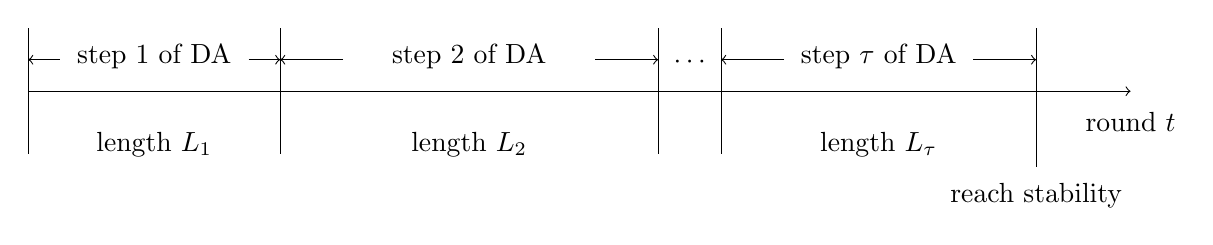
\begin{tikzpicture}[scale=0.8, every node/.style={node distance = 0.9cm}]


    \draw [->](5,0)--(22.5,0);
    \coordinate [label=round $t$](round) at(22.5,-0.8);
    

    \draw (5,1)--(5,-1);
    
    \draw [->](8.5,0.5)--(9,0.5);
    \draw [->](5.5,0.5)--(5,0.5);
    \coordinate [label=step $1$ of DA](s1) at(7,0.2);
    \coordinate [label=length $L_1$](s1R) at(7,-1.2);
    
    \draw (9,1)--(9,-1);
    
    \draw [->](10,0.5)--(9,0.5);
    \draw [->](14,0.5)--(15,0.5);
    \coordinate [label=step $2$ of DA](s2) at(12,0.2);
    \coordinate [label=length $L_2$](s2R) at(12,-1.2);
    
    \draw (15,1)--(15,-1);
    
    \coordinate [label=$\cdots$](cdots) at(15.5,0.2);
    \draw (16,1)--(16,-1);

    \draw [->](17,0.5)--(16,0.5);
    \draw [->](20,0.5)--(21,0.5);
    \coordinate [label=step $\tau$ of DA](stau) at(18.5,0.2);
    \coordinate [label=length $L_{\tau}$](stauR) at(18.5,-1.2);

    \draw (21,1)--(21,-1.2);
    
    \coordinate [label=reach stability](end) at(21,-2);

    \end{tikzpicture}

    \caption{A demonstration for the total horizon of Algorithm \ref{alg:decen}. The length $L_{\ell}$ of each step $\ell$ is $\max_{i\in[N]} 96{|S_{i,\ell}|\log T}/{\Delta^2}+2$, where $S_{i,\ell}$ denotes the set of arms who propose player $p_i$ at step $\ell$ following the offline DA algorithm.  
    }
    \label{fig:illustration}
\end{figure}


The total horizon $T$ in Algorithm \ref{alg:decen} can then be divided into several steps according to the DA algorithm. At each step $\ell$, each player $p_i$ attempts to pull the arm in $S_{i,\ell}$ in a round-robin way until it identifies the most-preferred one. 
According to Lemma \ref{lem:cen:ucblcb}, once an arm is deleted from the plausible set, then it is truly less-preferred. 
Further, based on Lemma \ref{lem:cen:pulltime}, each step $\ell$ would lasts for at most $\max_{i\in[N]}96|S_{i,\ell}|\log T/\Delta^2+2$ rounds, where the $2$ rounds are the time it takes for all players to detect the end of a step.   
Figure \ref{fig:illustration} gives an illustration for the total horizon of Algorithm \ref{alg:decen}. Formally, the regret can be decomposed as



\begin{align}
    \EE{\sum_{t=1}^T \bOne{{A}_i(t) \notin M^*}\mid \urcorner \cF } 
    &\le \sum_{\ell=1}^\tau \bracket{\max_{i\in[N]}|S_{i,\ell}|\cdot \frac{96\log T}{\Delta^2} +2 }\label{eq:decen:duetofigure}\\
    &= \sum_{\ell=1}^\tau \bracket{\max_{i\in[N]}(|R_{i,\ell}|+1)\cdot \frac{96\log T}{\Delta^2}+2} \notag \\
    &\le 2\sum_{\ell=1}^\tau \max_{i\in[N]}|R_{i,\ell}|\cdot \frac{96\log T}{\Delta^2} +2NK \label{eq:decen:duetoRmorethan1}\\
    &\le 2\sum_{\ell=1}^\tau \sum_{i\in[N]}|R_{i,\ell}|\cdot \frac{96\log T}{\Delta^2} +2NK \notag \\
    &\le \frac{192NK\log T}{\Delta^2} +2NK  \label{eq:decen:duetoRejectionAtMostNK}\,,
\end{align}
where Eq.\eqref{eq:decen:duetofigure} holds according to Lemma \ref{lem:cen:pulltime} and Figure \ref{fig:illustration}, Eq.\eqref{eq:decen:duetoRmorethan1} holds since $\max_{i}|R_{i,\ell}|\ge 1$ before the offline DA stops and $\tau\le NK$ as at each step at least one rejection happens (thus DA lasts for at most $NK$ steps before finding the stable matching), Eq.\eqref{eq:decen:duetoRejectionAtMostNK} holds since the number of all rejections is at most $NK$. 


\end{proof}







\begin{lemma}\label{lem:decen:sameP}
In Algorithm \ref{alg:decen}, for any arm $a_j\in \cK$ and round $t$, $P_{i,j}(t) = P_{i',j}(t)$ for any different players $p_i,p_{i'}$. 
\end{lemma}
\begin{proof} 

At the beginning, each player $p_i$ initializes $P_{i,j}=\cN$, thus the result holds. In the following rounds, player $p_i$ updates $P_{i,j}(t)$ only if it observes all players select the same arm for two consecutive rounds. Since the observations of all players are the same, they would update $P_{i,j}$ simultaneously. Above all, $P_{i,j}(t) = P_{i',j}(t)$ would always hold for any different player $p_i,p_{i'}$, arm $a_j$ and round $t$. 


\end{proof}




\subsection{Proof of Theorem \ref{thm:decen:strategy}}


\begin{proof}[Proof of Theorem \ref{thm:decen:strategy}]
According to the construction rule, $S_i$ is defined as the set of arms that can successfully accept player $p_i$ at the current round and still have the potential to be the most preferred one. 
So for any arm $a_j \notin S_i$, there must be $p_i \notin \ch_j(P_{i,j})$.  
This means that $p_i$ may be rejected and receive neither observation or reward when selecting $a_j$. So $p_i$ has no incentive to select arms beyond $S_i$. 

  
Recall that our ODA algorithm is an online version of the DA algorithm with the arm-side proposing. \citet[Theorem 3]{vaish2017manipulating} show that when a single player $p_i$ misreports an optimal manipulation as its preference ranking, i.e., under which manipulation the player can match an arm that has a higher preference ranking than that under any other manipulation by following DA, then the resulting matching of DA is still a stable matching. Since the original matching is the players' least preferred one, each player can match an arm in this new matching that is better than the arm in the original matching generated under the true preference ranking. 

  
\end{proof}








